\chapter{Results}

\textbf{REMAKE PLOTS WITH EPS ONCE THEY ARE READY}

Having constructed the theory of the physics and computation, we are in a position to discuss the results that come about from these reconstruction efforts. To discuss these results, we consider the methods in which a reconstruction technique can be considered successful. The easiest, and most useful parameter to check is the direction. Comparing the reconstructed direction with the true direction is done by computing the solid angle between the directions. Computing this is simple; suppose the reconstructed direction is $\vec{u}$ and the true direction is $\vec{v}$, then the solid angle is
\begin{equation}
  \alpha = \arccos(\vec{u}\cdot\vec{v})\, ,
\end{equation}
where we are assuming the directions are normalized to unit length. This solid angle can then be used to fill a histogram of a large number of trials to build a distribution. 

\section{Linefit}

The simplest method for reconstruction that has been discussed is the linear fit using the method of least squares. In figure \ref{fig:alpha_linefit} we see that this method provides a pretty decent first guess for a direction. The angular resolution seems to peak around a three degree resolution, and slowly falls off as we get further away from the truth. 

\begin{figure}[H]
  \centering
  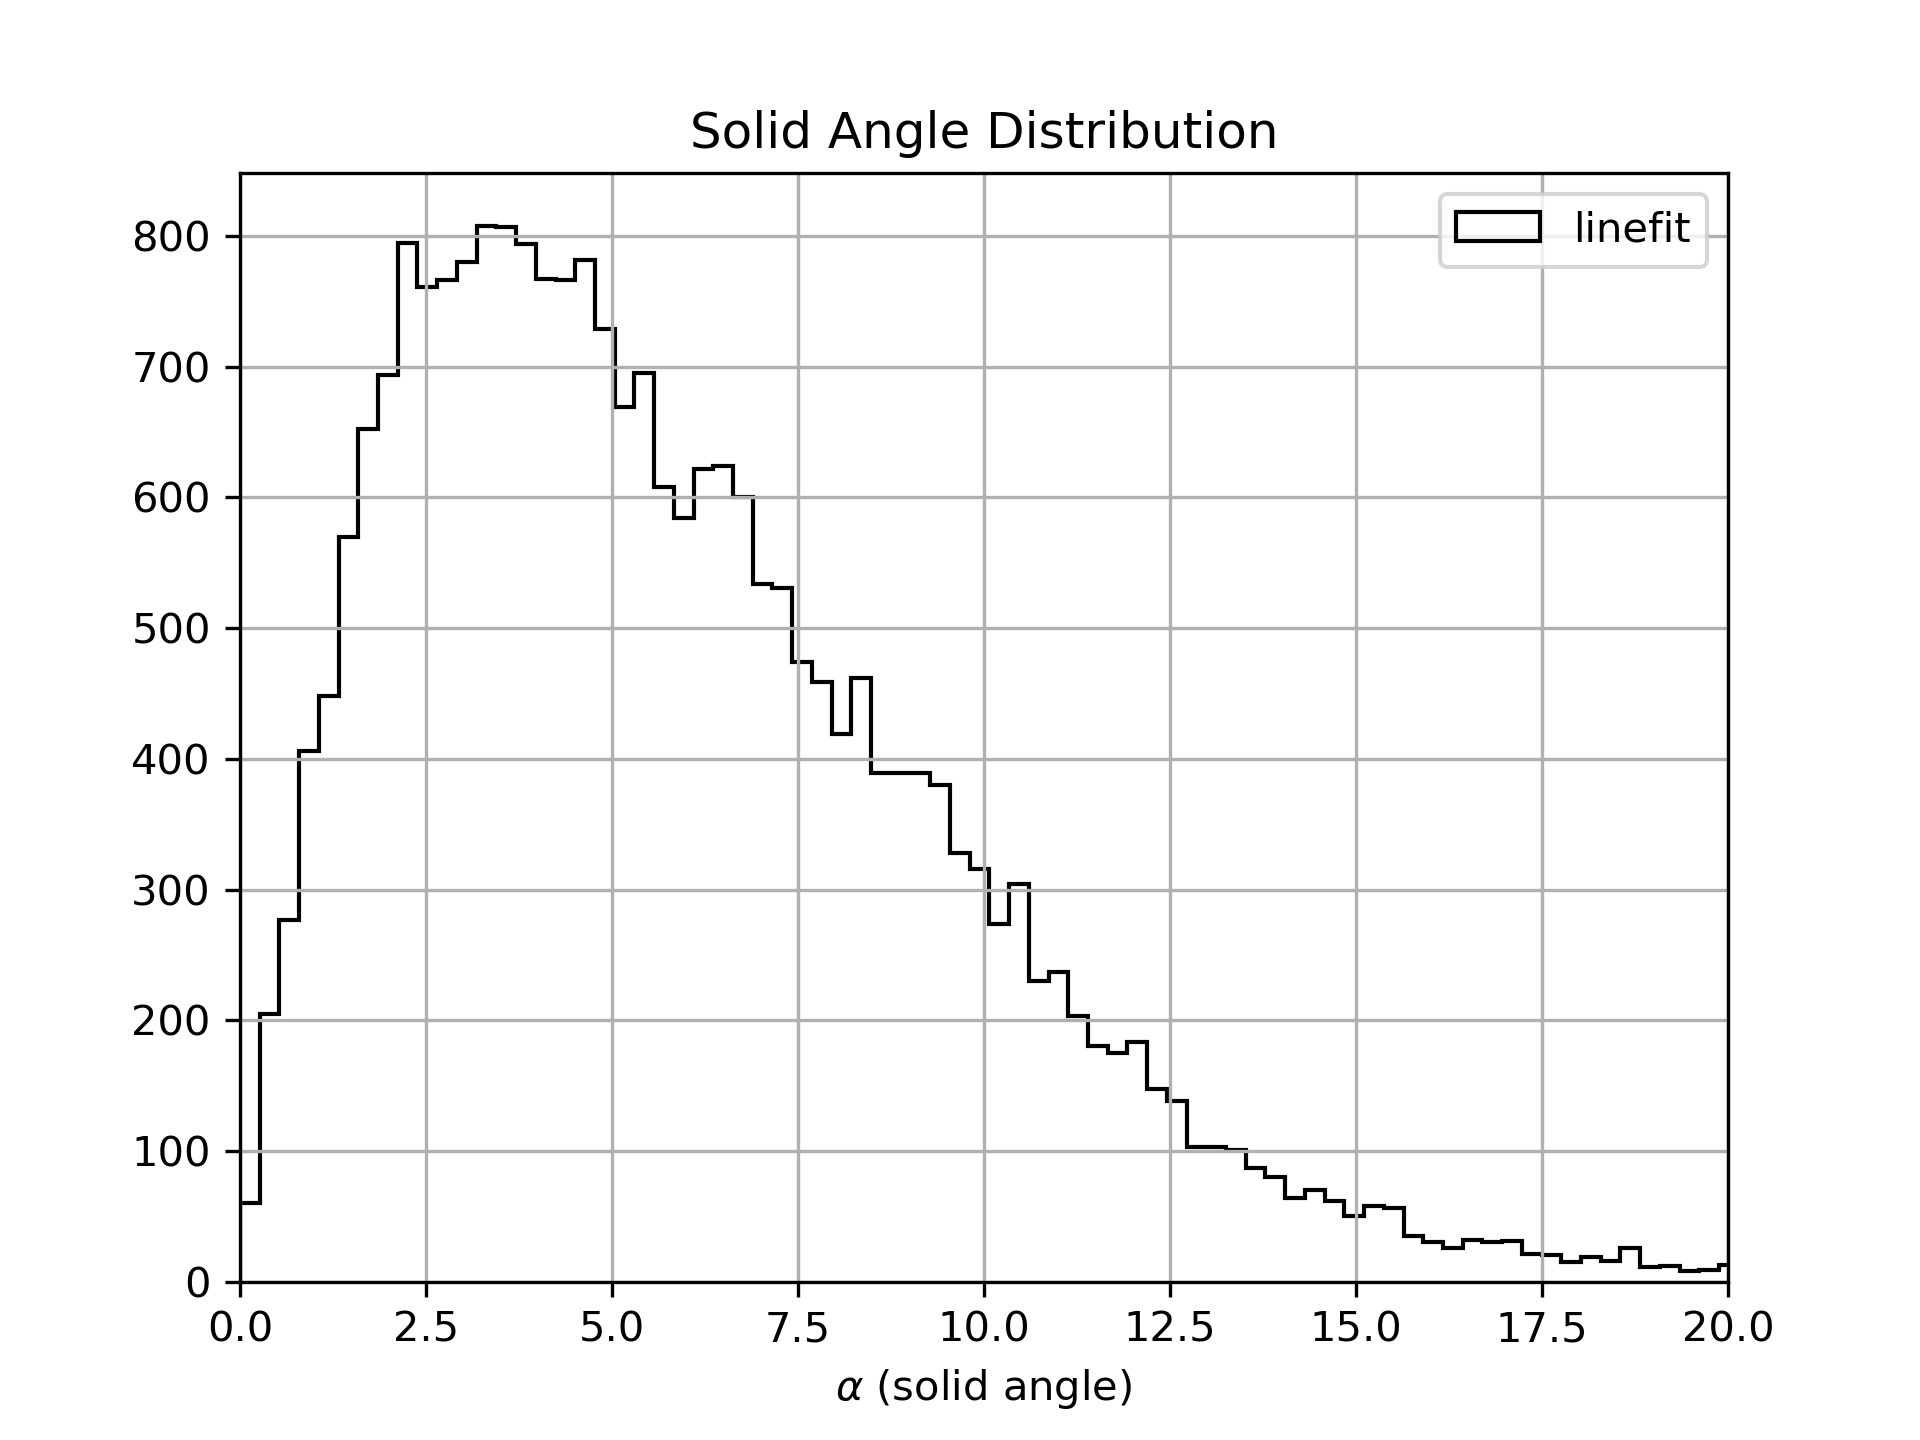
\includegraphics[width=12cm]{./Figures/reco_plots/alpha_dist_linefit_count.png}
  \caption{A distribution of the solid angles for reconstructed and true directions using the linefit method. The solid angle is given in degrees for clarity.}
  \label{fig:alpha_linefit}
\end{figure}

The quality of this reconstruction will inevitably affect the quality of the following reconstruction step, and as such should not be ignored. 

\section{Likelihood}

We can make a similar plot for the angular distribution of the reconstructed angle using the linefit as a seed to the likelihood algorithm. Looking at figure \ref{fig:alpha_llh} we see how well the likelihood reconstruction performs when using the linefit as a seed, but also how it compares to a perfect starting point, the true track information.

\begin{figure}[H]
  \centering
  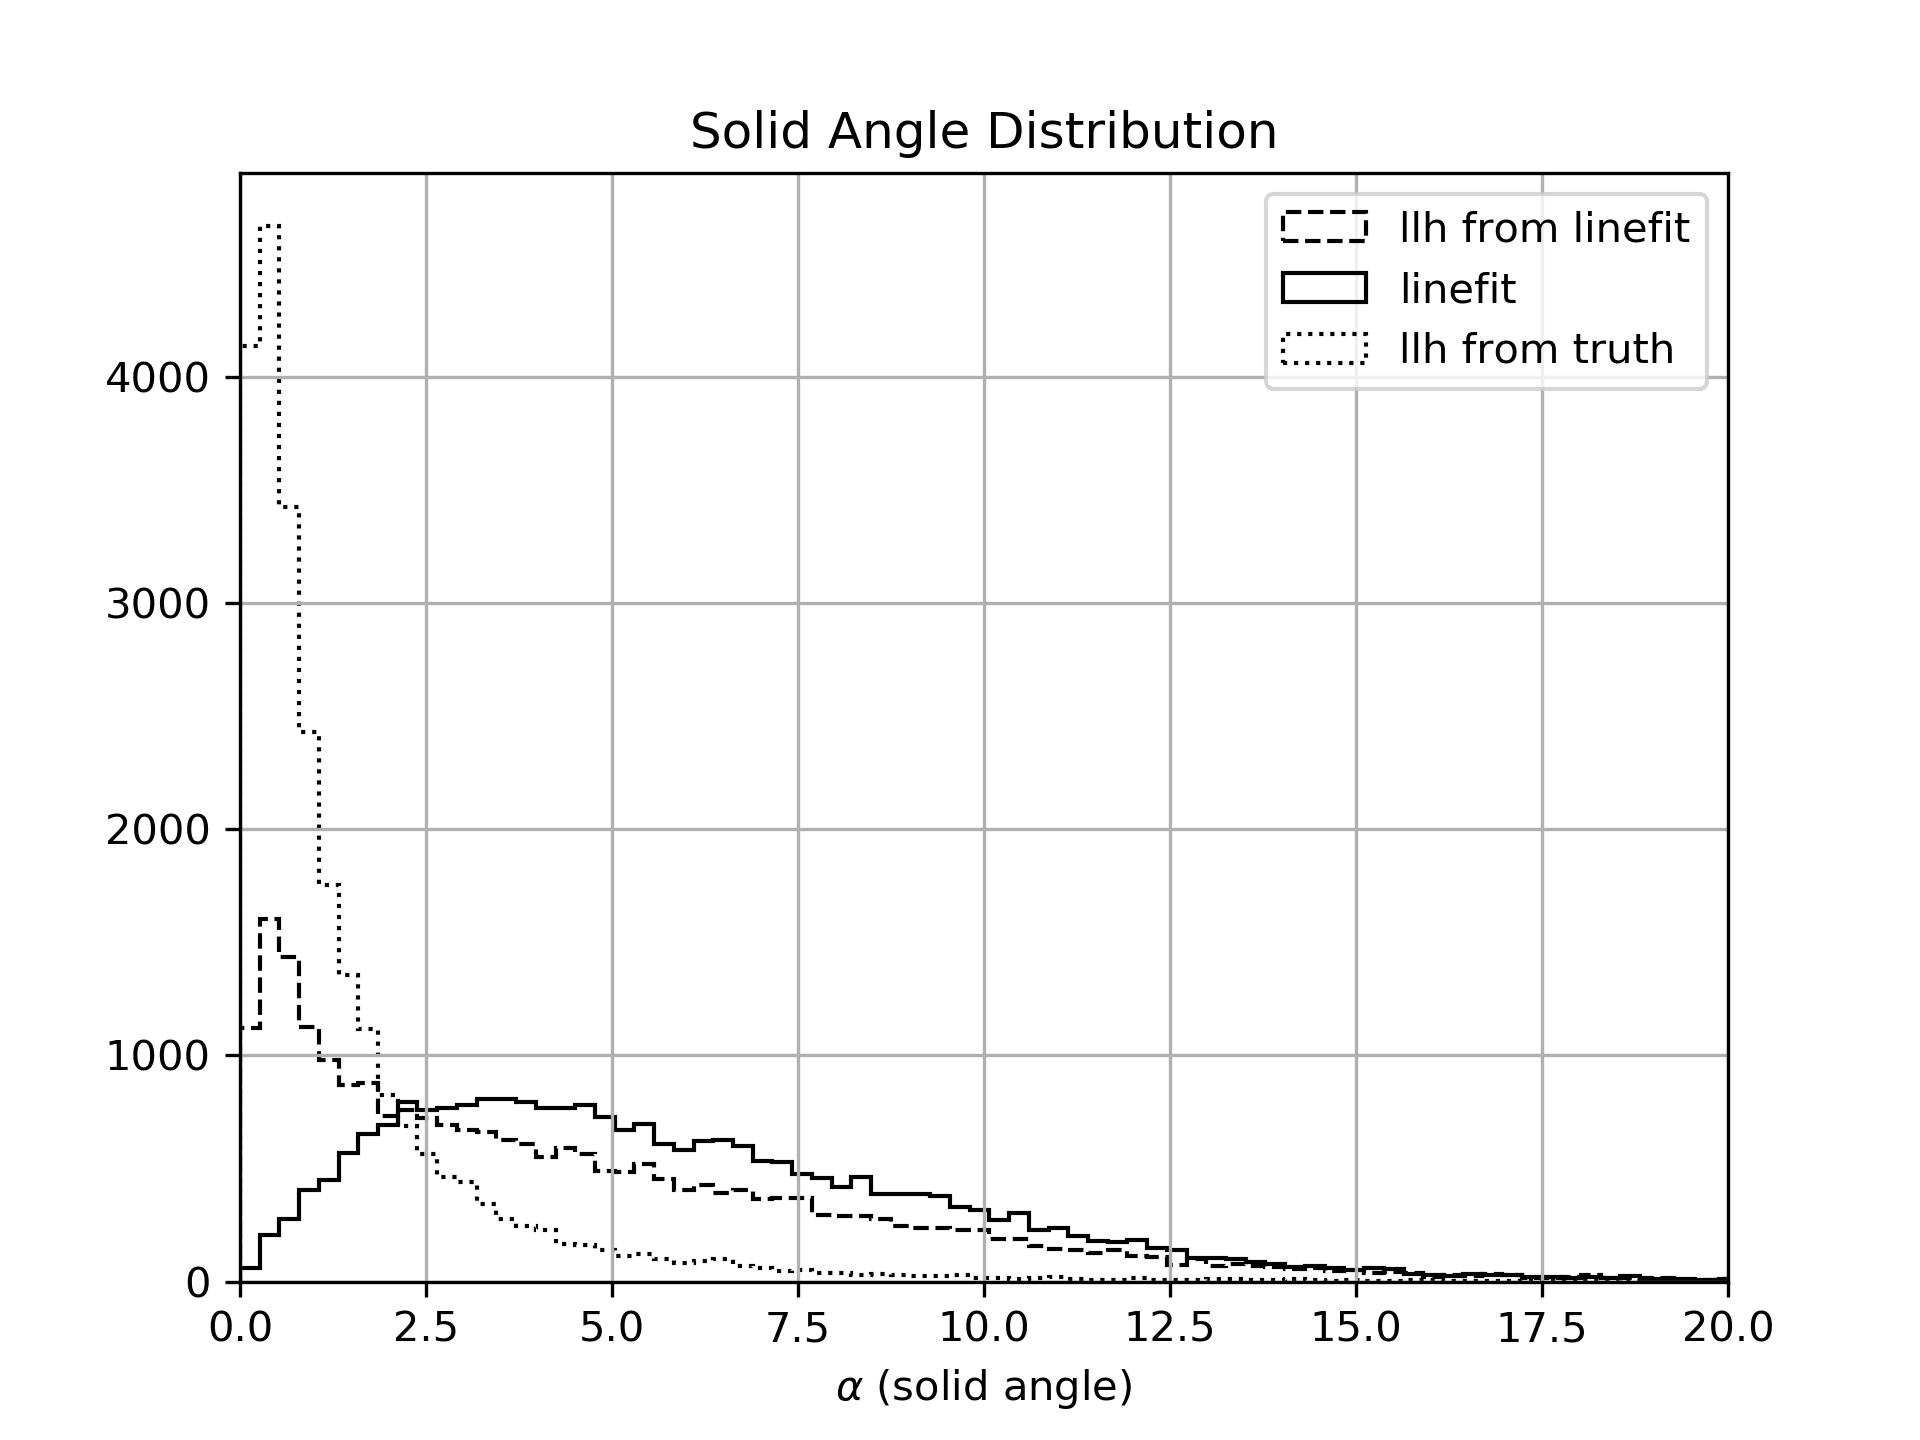
\includegraphics[width=12cm]{./Figures/reco_plots/alpha_dist_llh_count.png}
  \caption{A distribution of the solid angles for reconstructed and true directions using the likelihood method. The linefit reconstruction angular resolution is also plotted alongside a distribution for the likelihood given the true track as a starting point.}
  \label{fig:alpha_llh}
\end{figure}

Figure \ref{fig:alpha_llh} shows us that with perfect information, the likelihood reconstruction does pretty well. This effectively shows the upper limit to the performance of the reconstruction as it is, but also shows that there is plenty of room for improvement when starting at the linefit seed. It is relatively standard for reconstruction techniques to be highly dependent upon the initial conditions, as the technology used boils down to being a minimization of a multiparameter space. This effect is in full swing when we compare the two starting conditions, which emphasizes that another path to improving the reconstruction would be to improve the initial guess.

This resolution plot can also be represented by plotting the difference in the directional coordinates. As the directions are length one, we can seperate the azimuthal ($\phi$) and zenith ($\theta$) errors. Then, plotting the difference between the true azimuth/zenith and the reconstructed azimuth/zenith leads to figure \ref{fig:alpha_llh_sep}. 

\begin{figure}[H]
  \centering
  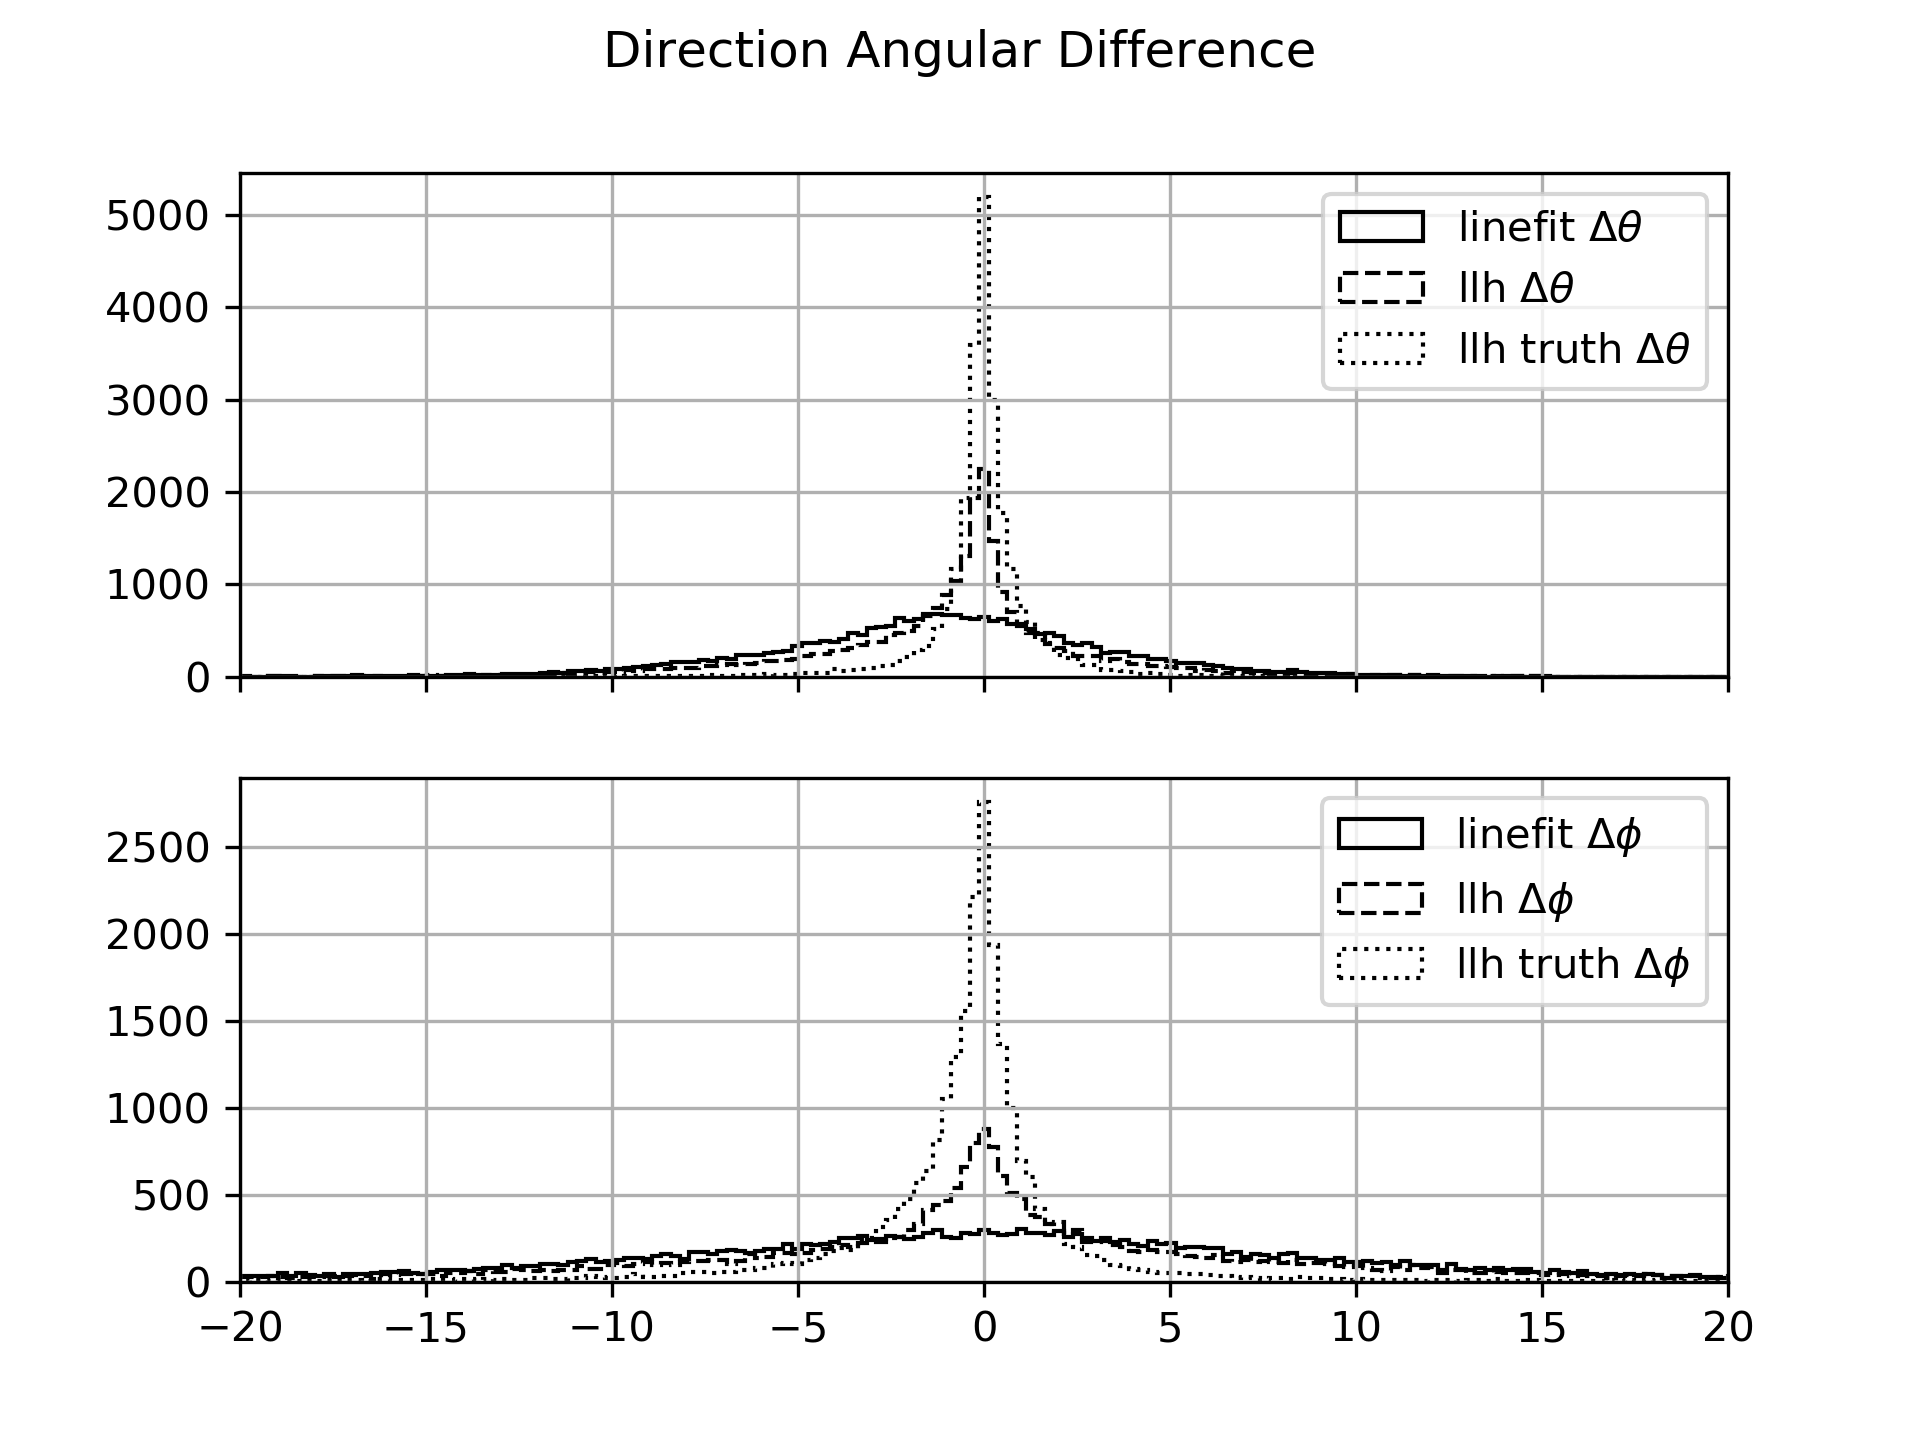
\includegraphics[width=12cm]{./Figures/reco_plots/angular_diff_dir.png}
  \caption{A distribution of the solid angles for reconstructed and true directions using the likelihood method seperated into zenith and azimuth components in degrees. \textbf{Above:} The zenith component distribution where $\Delta\theta = \theta_{\text{true}} - \theta_{\text{reco}}$ in the reconstruction process. \textbf{Below:} The azimuth component distribution where $\Delta\phi = \phi_{\text{true}} - \phi_{\text{reco}}$ in the reconstruction process.}
  \label{fig:alpha_llh_sep}
\end{figure}

The reconstruction still shows a similar shape that that observed in figure \ref{fig:alpha_llh}, as clearly the angular resolution in highly initial condition dependent. There is something of note in the zenth plot though ($\theta$), as there is a slight skewing towards negative $\Delta\theta$ values when using the linefit. This is due to the way the detector is simulated, since the current setup assumes IceCube-like DOMs which only face downward. As linefit is ignorant to the actual method in which light is emmitted from the track, this introduces a degeneracy in the fit that can push linefit towards a particular direction.

The resolution in the zenith angle seems to be slightly better than that of the azimuthal, which can be attributed to the geometry of the detector. In particular, the current geometry assumes vertical lines of detectors, which would expectedly perform better. These plots are in fact excellent for attempting to understand the effects of the geometry of the detector.

To test which initial parameter most affects the reconstruction, I started the reconstruction seed from two different initial states; fixing the starting vertex at the truth, and fixing the starting direction in the true direction. Using these initial conditions, a plot similar to figure \ref{fig:alpha_llh} could be created, and is in figure \ref{fig:alpha_llh_test}. As can be seen from the legend, there are a couple of variable seeds in this distribution, and the results seem to point towards the vertex resulting in the largest improvement in the resolution. This can come off as a bit surprising, especially when the parameter that is being plotted against is the direction resolution. The improvement does tell us where we need to improve the initial guess, and focusing on an improved vertex for the initial seed seems to be the way to go.

\begin{figure}[H]
  \centering
  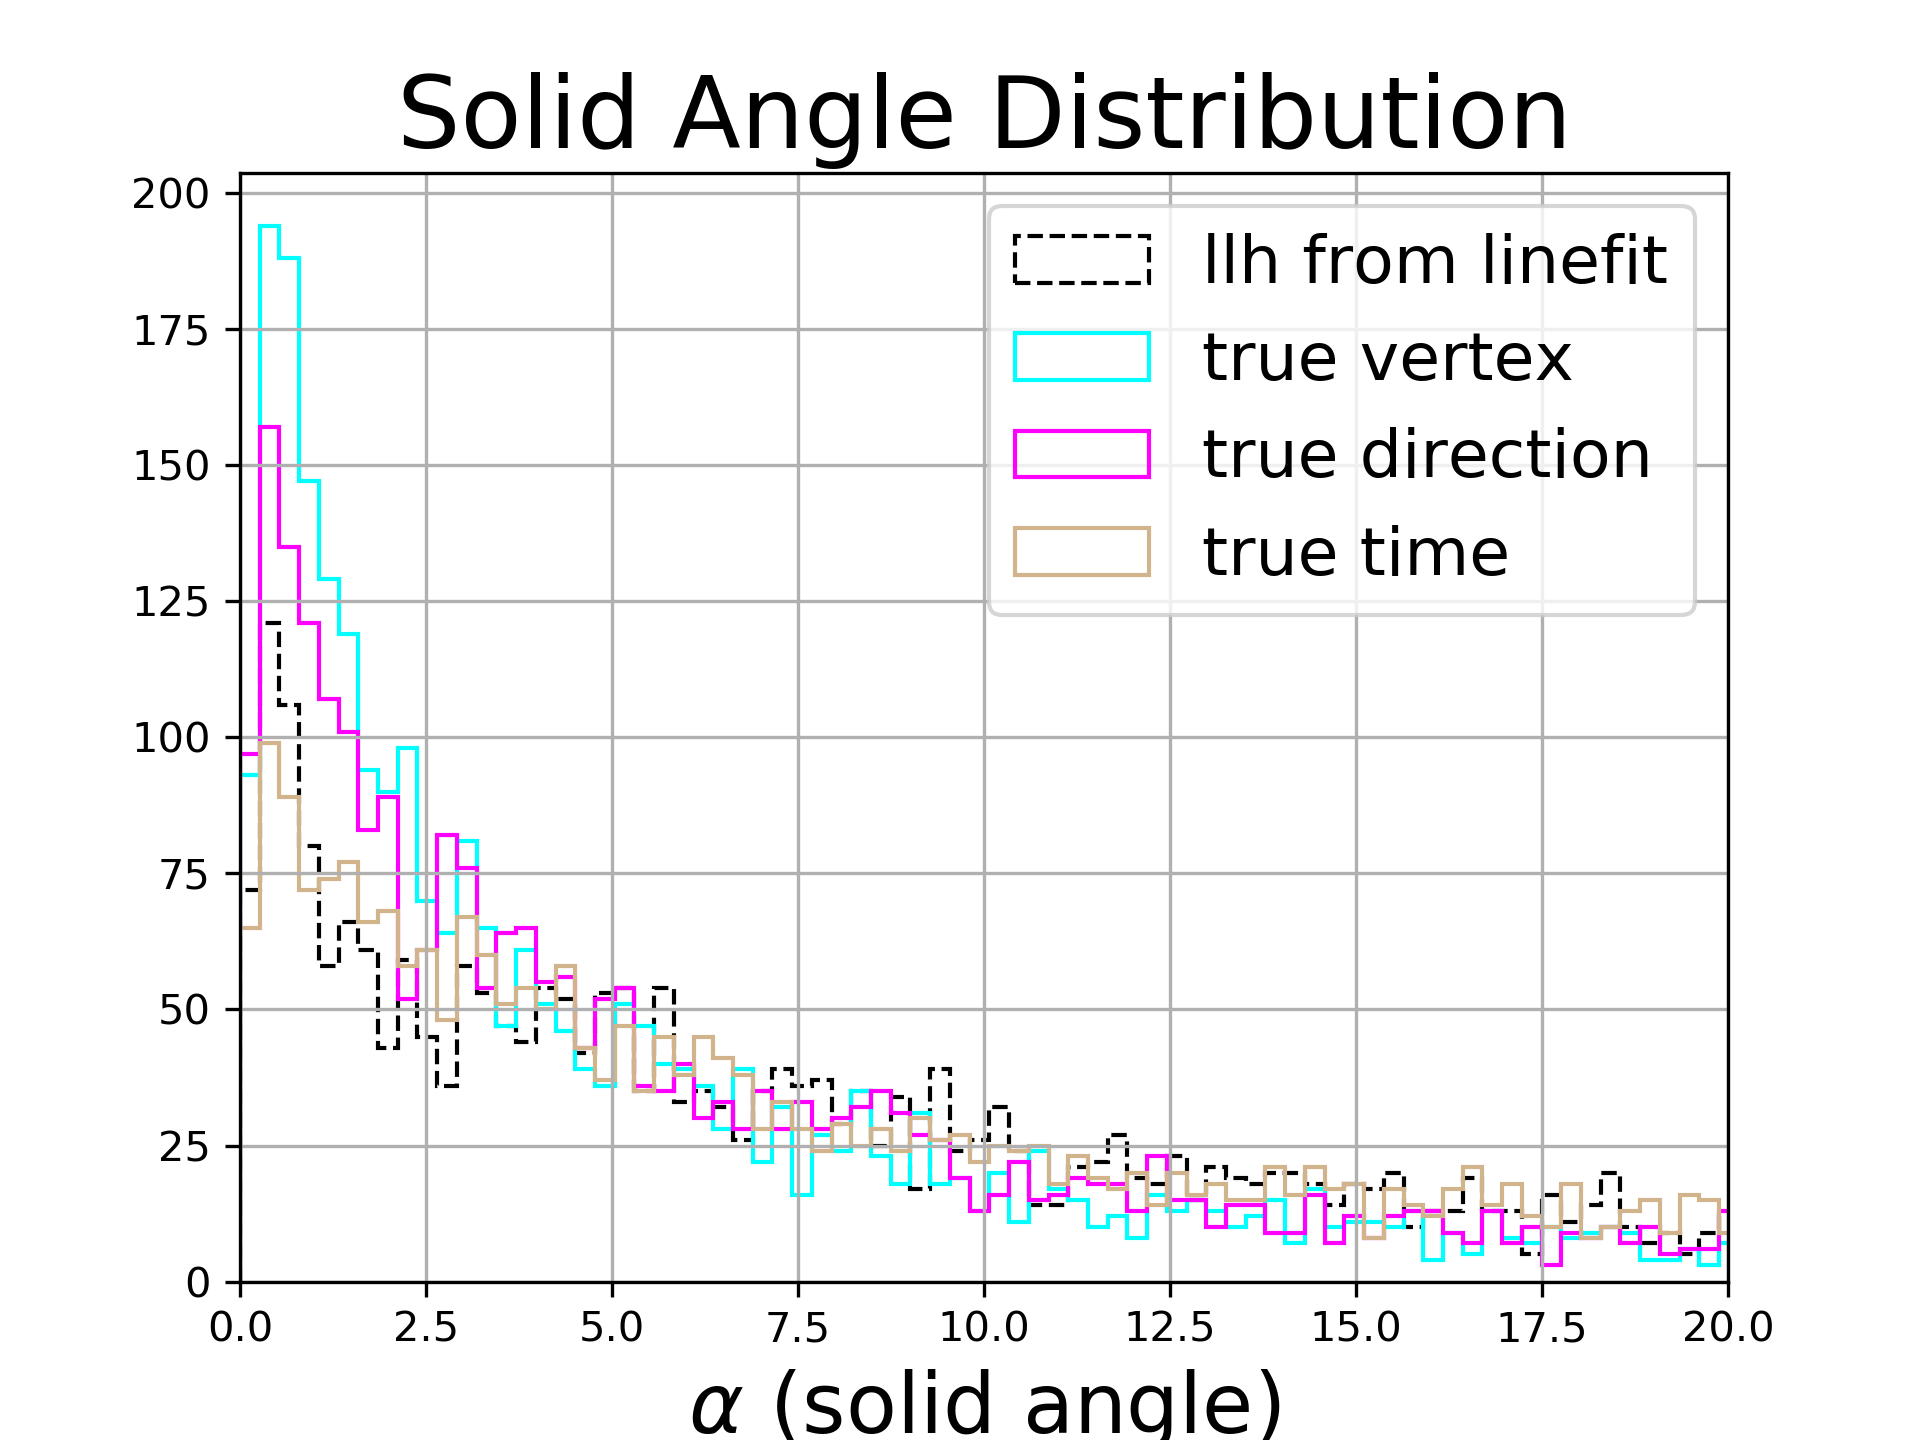
\includegraphics[width=12cm]{./Figures/reco_plots/alpha_dist_llh_seedcomparison.png}
  \caption{Similar to the distribution in figure \ref{fig:alpha_llh}, the angular resolution is plotted in degrees into a histogram. Here the initial starting conditions are grouped into the true vertex, true direction and only linefit, where the former are given linefit parameters for the remaining parameters.}
  \label{fig:alpha_llh_test}
\end{figure}

We can also check whether there is a correlation with the likelihood values and the reconstructed angular resolution ($\alpha$). To do so, we need a way to include both the final and initial likelihood values, as there can be a wide variety of ranges that a reconstruction can start and end at. For this reason, we consider plotting the ratio between the final negative loglikelihood value and the initial, $\ell_{f}/\ell_{i}$. Thus, a smaller value denotes a larger improvement in the likelihood value. On the other hand, any value above one denotes a drop in quality of fit. This plot is made in figure \ref{fig:alpha_llhratio_comp}.

\begin{figure}[H]
  \centering
  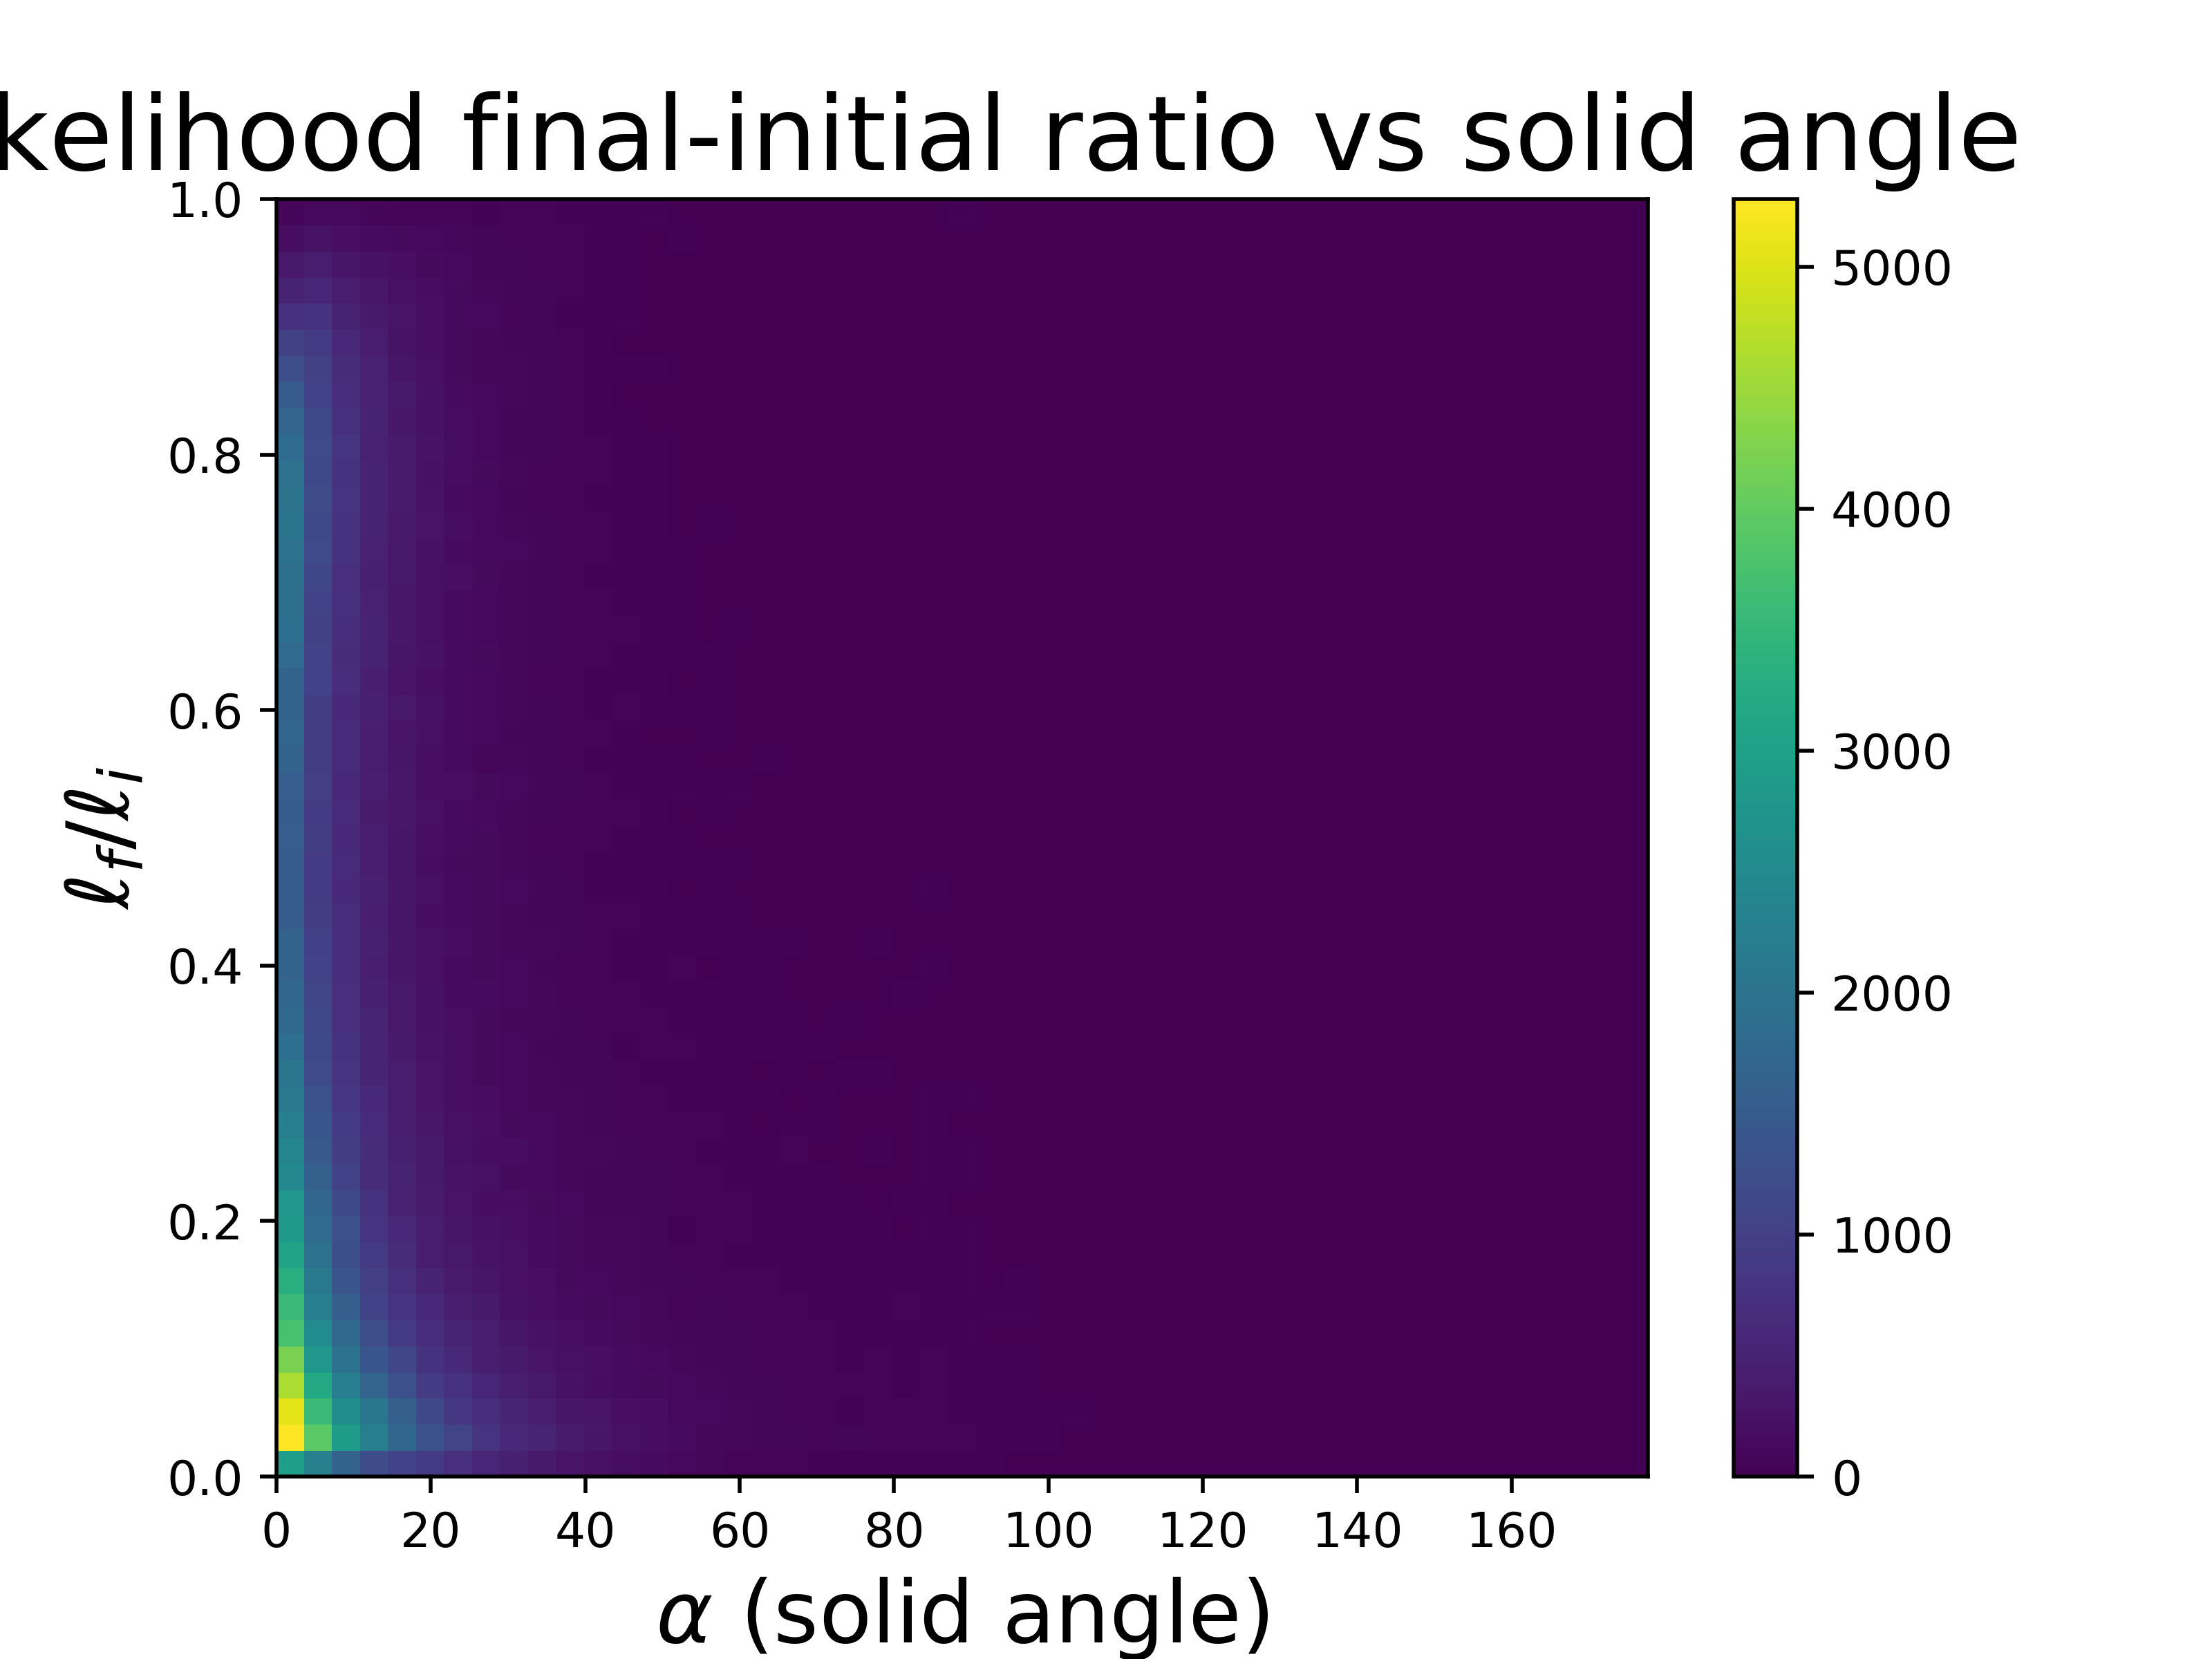
\includegraphics[width=12cm]{./Figures/reco_plots/alpha_dist_vs_llhratio_heat.png}
  \caption{We plot the likelihood ratio $\ell_{f}/\ell_{i}$ against the final reconstructed angular resolution using a heatmap. }
  \label{fig:alpha_llhratio_comp}
\end{figure}

Referring to figure \ref{fig:alpha_llhratio_comp}, we see that the events are bunching up near a small ratio of $\ell_{f}/\ell_{i}$ and small error in the solid angle $\alpha$. This could point to a correlation between the increase in the quality of the fit and the increase in the direcitonality of the reconstructed track. There could still be some hidden biases here that are being unaccounted for, such as reconstruction angles that begin close to the truth only changing in small amounts but having massive likelihood value swings. For this reason, we need to check for sure that there are no hidden biases in both $\ell_{f}$ against $\ell_{i}$ and $\alpha_{f}$ against $\alpha_{i}$.

\begin{figure}[ht]
  \begin{minipage}[b]{0.48\linewidth}
    \centering
    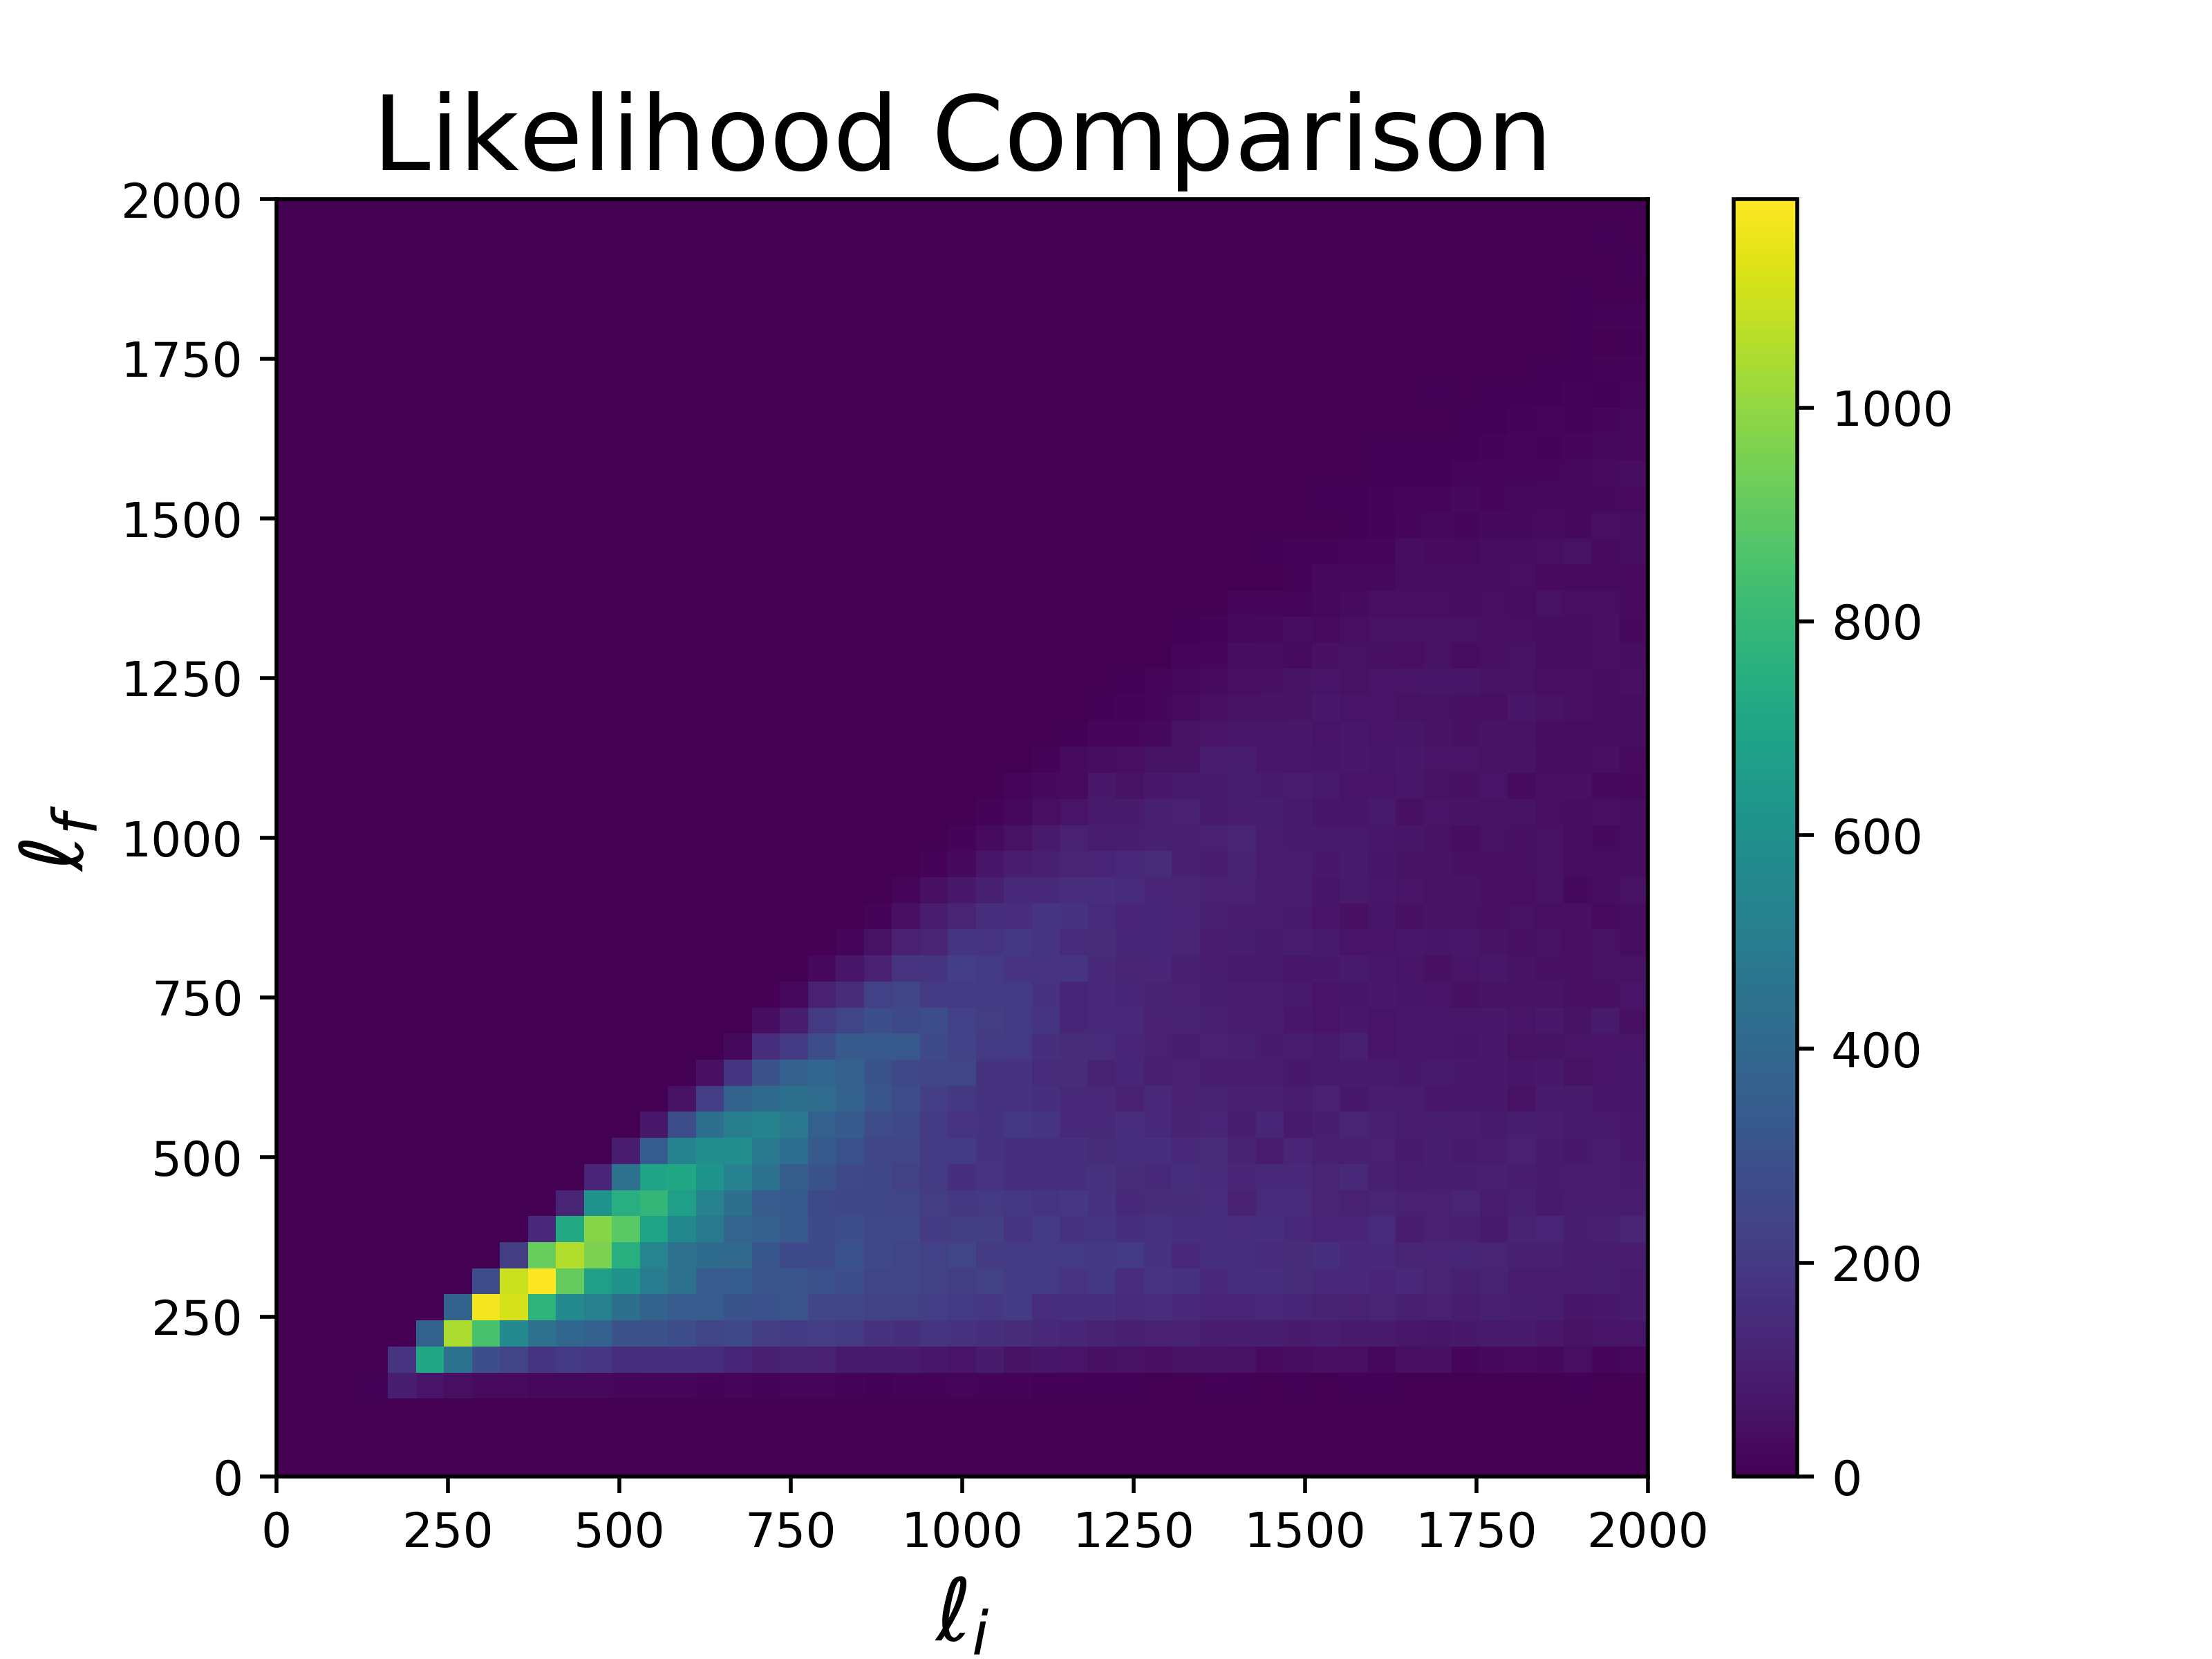
\includegraphics[width=\textwidth]{./Figures/reco_plots/llhratio_comp_heat.png}
    \caption{Correlation heatmap between the initial negative loglikelihood value and the final negative loglikelihood.}
    \label{subfig:llh_heat}
  \end{minipage}
  \hspace{0.1cm}
  \begin{minipage}[b]{0.48\linewidth}
    \centering
    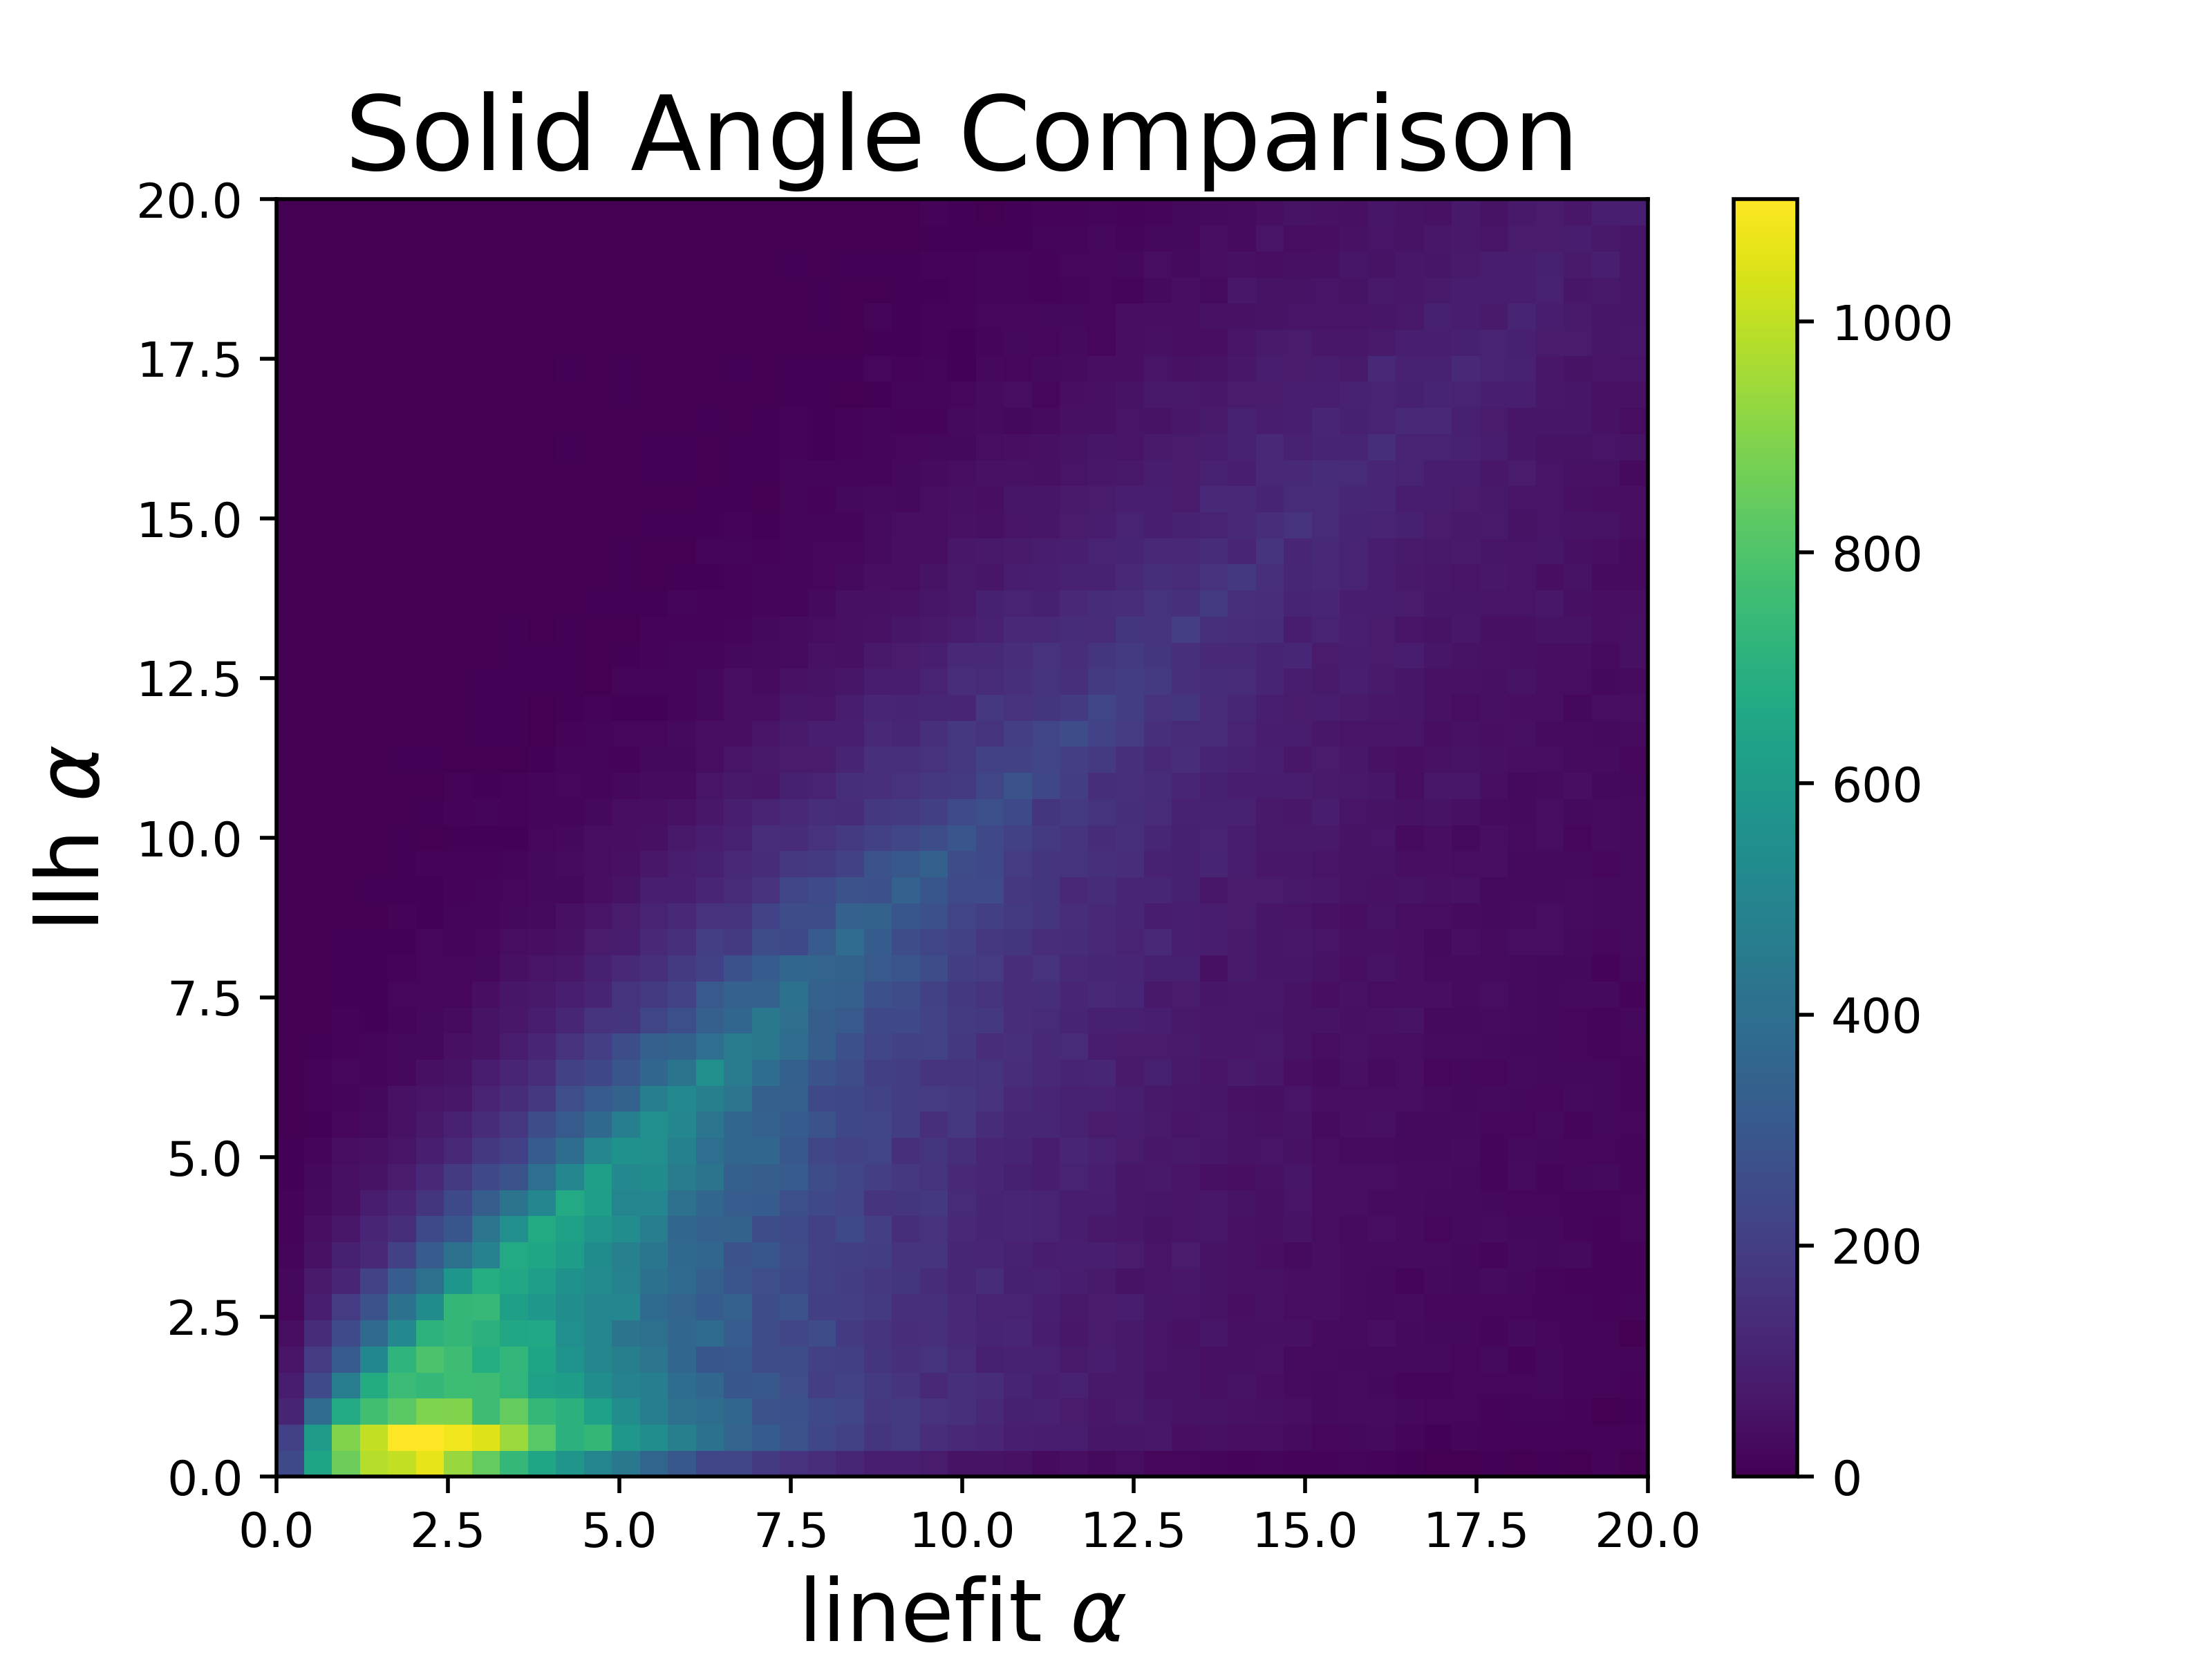
\includegraphics[width=\textwidth]{./Figures/reco_plots/alpha_dist_comp_heat.png}
    \caption{Correlation map of the final reconstructed angular resolution and the initial angular resolution.}
    \label{subfig:alpha_heat}
  \end{minipage}
\end{figure}

Looking at figures \ref{subfig:llh_heat} and \ref{subfig:alpha_heat}, we can see that the reconstruction is behaving as one would expect. For both plots, the $y=x$ diagonal line would symbolize neither improvement nor regression, and anything below would suggest improvement. In both figures majority of the points end up below this line encouraging the 


computation time

what affects the reco the most


